\documentclass[runningheads]{llncs}

\usepackage{amsmath}
\usepackage{booktabs}
\usepackage{graphicx}
\usepackage{url}

\graphicspath{{../figures/}}

\begin{document}

\title{Robustness of Hierarchy-Aware CLIP Adaptation Under Noisy Taxonomic Supervision}
\titlerunning{Hierarchy-Aware CLIP Under Noisy Taxonomies}

\author{Submission Report}
\authorrunning{VLM Fine-Tuning Experiments}
\institute{GitHub repository: \url{https://github.com/manuvikash/VLM-finetune}}

\maketitle

\begin{abstract}
Vision-language models are often adapted to domain-specific recognition tasks
using labels that are organized in a taxonomy. In practice, these taxonomies
are rarely perfect: parent labels can be missing, ambiguous, inconsistently
mapped across sources, or systematically wrong. This paper studies how
hierarchy-aware adaptation of CLIP behaves when parent-class supervision is
corrupted. We construct a three-level CIFAR-100 hierarchy with 100 leaf
classes, 20 parent classes, and six top-level domains, then compare zero-shot
CLIP, flat supervised adaptation, clean hierarchy-aware adaptation, and noisy
hierarchy-aware adaptation. To make a multi-seed degradation study feasible on
a commodity 4GB GPU, we cache OpenCLIP ViT-B/32 image embeddings and train a
lightweight residual adapter with leaf and parent classification heads. The
hierarchy objective combines direct parent classification with a differentiable
leaf-to-parent consistency loss, allowing parent supervision to influence the
fine-grained decision boundary. Across three seeds, flat adaptation reaches
73.15\% leaf accuracy and clean hierarchy-aware adaptation reaches 73.20\%.
Uniform parent-label corruption is relatively benign, retaining 71.19\% leaf
accuracy even at full corruption. However, structured taxonomy noise is far
more damaging: in-domain corruption drops to 63.97\%, while cyclic systematic
corruption drops to 47.93\%. These results show that the danger in hierarchical
supervision is not only the amount of taxonomy noise, but whether the noise is
coherent enough to teach the model a wrong ontology.

\keywords{vision-language models \and CLIP \and hierarchical classification
\and noisy labels \and taxonomy \and robustness \and reproducibility}
\end{abstract}

\section{Introduction}
Large vision-language models (VLMs) such as CLIP are widely used as foundation
models for downstream visual recognition. A common adaptation strategy is to
freeze or lightly tune the visual backbone, then train task-specific heads on
top of the learned image representation. Many real classification tasks are
not flat, however. Product catalogs, species datasets, medical image
ontologies, and remote-sensing taxonomies all organize labels into a hierarchy.
For example, an image may be labeled as a fine-grained leaf class such as
``pickup truck,'' a parent class such as ``vehicle,'' and a broader top-level
domain such as ``object'' or ``scene.''

Hierarchical supervision can provide useful inductive bias. If a model
confuses two leaf classes under the same parent, the error is usually less
severe than confusing classes across unrelated parents. A parent-level loss can
encourage features that respect this structure and may improve calibration,
top-k behavior, or robustness when leaf labels are sparse. Yet this benefit
comes with a practical risk. Real-world taxonomies are often noisy. Parent
classes may be assigned by separate annotators, inherited from legacy data
sources, or merged from incompatible schemas. In such cases, hierarchy-aware
training can inject supervision that conflicts with the leaf task.

This paper studies the robustness of hierarchy-aware CLIP adaptation under
controlled taxonomy noise. The goal is not simply to show whether hierarchy
helps on clean CIFAR-100, but to identify when hierarchical supervision becomes
harmful. We focus on three questions:
\begin{enumerate}
\item Does hierarchy-aware adaptation improve over flat supervised adaptation?
\item How does leaf accuracy degrade as parent-label corruption increases?
\item Are structured taxonomy errors more damaging than random parent noise?
\end{enumerate}

The main contribution is an end-to-end reproducible experiment pipeline that
builds a CIFAR-100 hierarchy, runs multi-seed noise sweeps, exports paper-ready
figures and CSV tables, and provides a Springer-format final report. The
empirical finding is clear: hierarchy-aware adaptation is robust to diffuse
uniform parent noise, but vulnerable to coherent systematic noise. The
expanded analysis also shows that calibration, semantic error distance,
parent-level collapse, and per-parent sensitivity reveal failure modes that are
not visible from leaf accuracy alone.

\section{Related Work}
CLIP introduced contrastive language-image pretraining at web scale, enabling
strong zero-shot transfer through natural language prompts \cite{radford2021clip}.
OpenCLIP provides open implementations and pretrained checkpoints that make
CLIP-style models practical for research use \cite{ilharco2021openclip}.
Because full fine-tuning of VLMs can be expensive, downstream adaptation often
uses linear probing, adapters, prompt tuning, or partial fine-tuning. These
methods trade off computational cost and task-specific flexibility.

Hierarchical classification has a long history in computer vision and machine
learning, with surveys emphasizing that the hierarchy can affect both model
training and evaluation \cite{silla2011survey}. Instead of treating all errors
equally, hierarchical methods exploit relationships among labels. Some
approaches modify the loss, some constrain predictions to respect a tree, and
others evaluate predictions with hierarchy-aware distances. A key motivation
is that semantic structure can regularize learning and provide more informative
error signals than flat classification alone.

Noisy-label learning is also closely related. In standard noisy-label settings,
the class label itself may be corrupted, and prior work has proposed loss
correction methods that estimate or compensate for label-transition noise
\cite{patrini2017noise}. This work differs in that the leaf label remains
clean while the auxiliary parent label is corrupted. The setting is common in
practice: a fine label may be curated manually while higher-level metadata is
inherited from a weak or inconsistent taxonomy. This makes the problem
especially subtle, because the primary target is correct but the auxiliary
supervision can still damage the learned representation. The structured noise
conditions also connect to shortcut-learning analyses: a model can exploit a
spurious but coherent signal when it is predictive during training, even if the
signal encodes the wrong abstraction \cite{geirhos2020shortcut}.

\section{Methodology}
\subsection{Dataset Construction}
The data pipeline converts CIFAR-100 into a three-level hierarchy. CIFAR-100
contains 100 fine classes and 20 coarse superclasses \cite{krizhevsky2009learning}.
We use each fine class as a leaf label and each coarse superclass as a parent
label. A top-level domain is added manually for each parent group, yielding
paths of the form:
\begin{equation}
\mathrm{domain} \rightarrow \mathrm{parent} \rightarrow \mathrm{leaf}.
\end{equation}
The full official CIFAR-100 split is used: 50,000 training images and 10,000
test images. This avoids ambiguity introduced by random train-test splits and
makes the experiment easier to reproduce.

\subsection{Model Architecture}
The visual backbone is OpenCLIP ViT-B/32 with OpenAI pretrained weights. In the
main sweep, image embeddings are extracted once and L2-normalized. Cached
features allow many taxonomy-noise configurations to be evaluated without
repeatedly running the vision transformer. This design is computationally
important for commodity hardware, but it still allows a trainable shared
representation through a residual adapter:
\begin{equation}
h(x) = z(x) + \mathrm{LN}(W_2\,\mathrm{GELU}(W_1z(x))),
\end{equation}
where $z(x)$ is the frozen CLIP image embedding. The adapter output $h(x)$ is
fed to a leaf head. In hierarchy-aware runs, it is also fed to a parent head.
The flat model and hierarchy-aware model therefore share the same feature
cache and adapter family; the difference is the presence or absence of the
hierarchy loss.

\subsection{Training Objectives}
The flat adaptation objective is standard leaf cross entropy:
\begin{equation}
\mathcal{L}_{flat} = \mathrm{CE}(y,\hat{y}),
\end{equation}
where $y$ is the leaf label and $\hat{y}$ is the leaf prediction.

The hierarchy-aware objective adds parent supervision:
\begin{equation}
\mathcal{L} =
\mathrm{CE}(y,\hat{y}) +
\lambda\left[(1-\alpha)\mathrm{CE}(p,\hat{p}) +
\alpha\mathrm{CE}(p,g(\hat{y}))\right].
\end{equation}
Here $p$ is the parent target, $\hat{p}$ is the parent-head prediction, and
$g(\hat{y})$ aggregates leaf logits into parent logits using parent-wise
log-sum-exp. This aggregation makes the auxiliary parent target act directly
on the leaf decision boundary. Without this coupling, a frozen-feature model
with independent heads can absorb parent-label noise in the parent head while
leaving leaf predictions almost unchanged. We use $\lambda=1.0$ and
$\alpha=0.8$ in the final sweep.

\subsection{Taxonomy Noise Models}
Only training parent labels are corrupted. Leaf labels, validation targets, and
test targets remain clean. Three noise mechanisms are studied:
\begin{itemize}
\item \textbf{Uniform noise:} with probability $\rho$, replace the true parent
with a uniformly sampled different parent.
\item \textbf{In-domain noise:} with probability $\rho$, replace the true
parent with another parent that shares the same top-level domain when such a
parent exists. This simulates plausible taxonomy confusion among related
groups.
\item \textbf{Cyclic noise:} with probability $\rho$, replace the true parent
with the next parent in a deterministic sorted cycle. This simulates a coherent
schema mapping error.
\end{itemize}
The corruption fraction $\rho$ is swept over
$\{0.0,0.05,0.1,0.2,0.3,0.5,0.7,1.0\}$.

\section{Experiments}
\subsection{Baselines}
Four primary conditions are evaluated. The first is zero-shot CLIP, using text
prompts of the form ``a photo of a \{class\}.'' The second is flat supervised
adaptation, which trains the residual adapter and leaf head with leaf labels
only. The third is hierarchy-aware adaptation with clean parent labels. The
fourth is hierarchy-aware adaptation with corrupted parent labels.

\subsection{Hyperparameters}
All supervised adapter experiments are run with three seeds: 42, 123, and 456.
The adapter is trained for 30 epochs with AdamW, learning rate $10^{-3}$,
weight decay $10^{-4}$, batch size 8192, adapter width 256, and dropout 0.05.
The feature extraction batch size is 256. All experiments are run with
Weights \& Biases disabled and write deterministic JSON rows to
\texttt{runs/results.json}. In addition to aggregate metrics, the rerun used
for this report logs \texttt{runs/per\_parent\_metrics.csv}, which records
leaf and parent accuracy for each true parent group, seed, corruption type, and
noise fraction.

\subsection{Metrics}
We report six metrics. Leaf accuracy is the primary fine-grained top-1 metric.
Top-5 accuracy measures whether the correct leaf appears among the five most
likely predictions. Parent accuracy measures whether the predicted parent is
correct, either from the parent head or from the predicted leaf's canonical
parent. Hierarchical distance measures tree distance between predicted and
true leaves: 0 for correct leaf, 2 for same-parent mistakes, 4 for same-domain
mistakes, and 6 for cross-domain mistakes. Severity-weighted accuracy gives
1.0 credit for a correct leaf, 0.5 credit for a wrong leaf under the same
parent, and 0.0 otherwise. Expected calibration error (ECE) is computed with
15 equal-width confidence bins \cite{guo2017calibration}.

\section{Results}
\subsection{Main Results}
Table~\ref{tab:main} summarizes the main comparison. Zero-shot CLIP obtains
56.05\% leaf accuracy. Both supervised adapters provide a large gain, reaching
approximately 73\% leaf accuracy. Clean hierarchy-aware adaptation is
statistically similar to flat adaptation in leaf accuracy, but it improves
hierarchical distance, severity-weighted accuracy, and calibration. Under
20\% uniform parent noise, leaf accuracy falls modestly to 72.56\%, but ECE
increases from 0.0179 to 0.0692. This indicates that mild taxonomy noise may
leave top-1 predictions mostly intact while still degrading confidence quality.

\begin{table}
\centering
\caption{Main results on the full CIFAR-100 hierarchy. Mean $\pm$ standard deviation is reported across three seeds where applicable.}
\label{tab:main}
\begin{tabular}{lrrrrrr}
\toprule
Condition & Leaf & Top-5 & Parent & H-Dist & Sev-W & ECE \\
\midrule
Zero-shot CLIP & 56.05 & 81.95 & 70.76 & 1.664 & 63.41 & 0.129 \\
Flat adapter & 73.15 & 93.46 & 83.12 & 0.972 & 78.14 & 0.025 \\
Hierarchy, clean & 73.20 & 93.39 & 79.34 & 0.960 & 78.33 & 0.018 \\
Hierarchy, uniform 20\% noise & 72.56 & 92.96 & 78.65 & 0.998 & 77.60 & 0.069 \\
\bottomrule
\end{tabular}
\end{table}

\subsection{Leaf-Accuracy Degradation by Noise Type}
The central result is shown in Fig.~\ref{fig:noise_by_type} and
Table~\ref{tab:noise_type}. Uniform noise is surprisingly robust. Even when
every training parent label is replaced by a random wrong parent, leaf accuracy
remains 71.19\%, only about two percentage points below the clean
hierarchy-aware result. In-domain noise is more damaging, reducing leaf
accuracy to 63.97\% at full corruption. Cyclic noise is most harmful, dropping
to 47.93\% at full corruption.

\begin{figure}
\centering
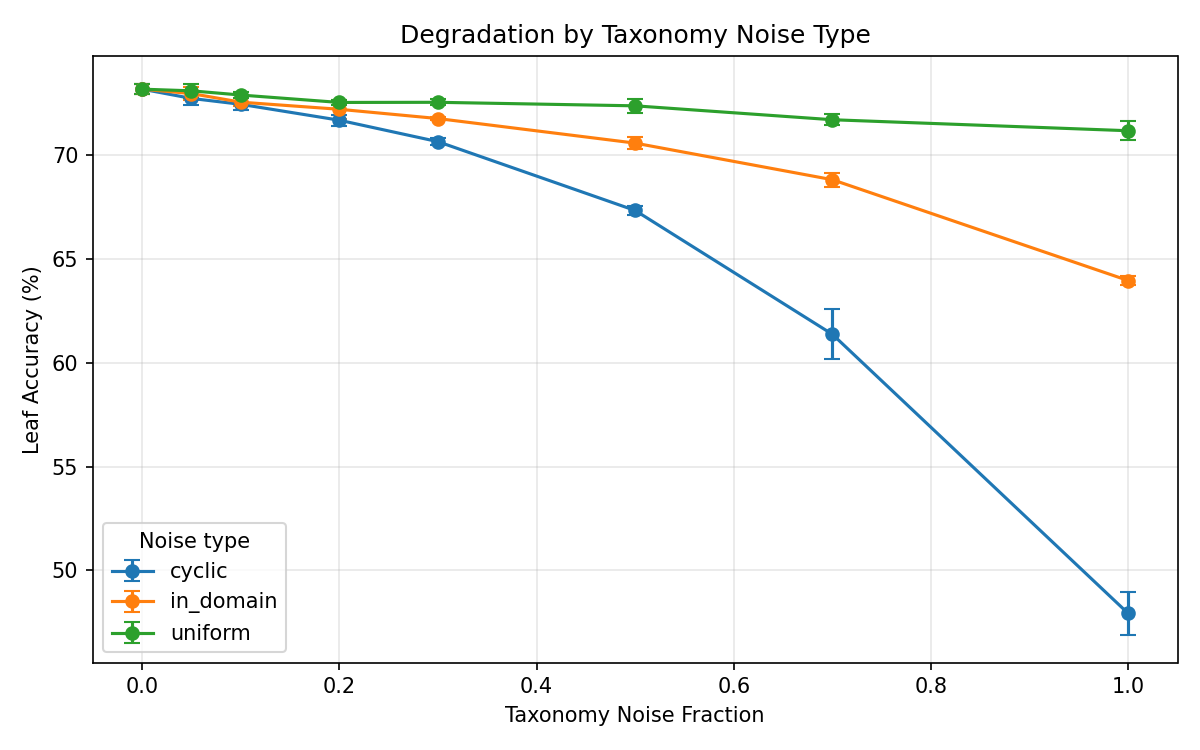
\includegraphics[width=0.88\textwidth]{noise_degradation_by_type.png}
\caption{Leaf-accuracy degradation by taxonomy noise type. Error bars show standard deviation across three seeds.}
\label{fig:noise_by_type}
\end{figure}

\begin{table}
\centering
\caption{Leaf accuracy under parent-label corruption.}
\label{tab:noise_type}
\begin{tabular}{lrrrr}
\toprule
Noise type & 0\% & 20\% & 50\% & 100\% \\
\midrule
Uniform & 73.20 & 72.56 & 72.39 & 71.19 \\
In-domain & 73.20 & 72.23 & 70.60 & 63.97 \\
Cyclic & 73.20 & 71.70 & 67.35 & 47.93 \\
\bottomrule
\end{tabular}
\end{table}

Figure~\ref{fig:delta} shows the same result as a delta from the clean
hierarchy baseline. This representation makes the severity of systematic
noise easier to read: cyclic corruption costs more than 25 percentage points
at full corruption, while uniform corruption costs only about two percentage
points. The delta plot is especially useful because the three curves share the
same clean baseline at zero noise.

\begin{figure}
\centering
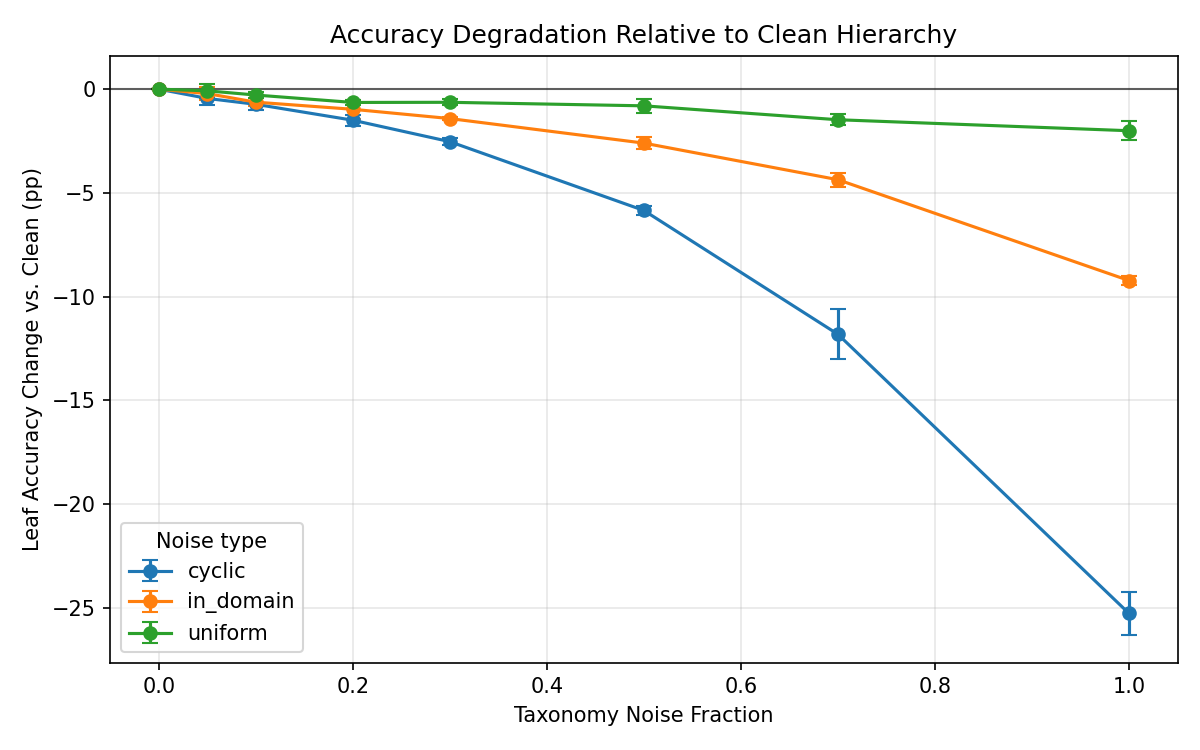
\includegraphics[width=0.88\textwidth]{accuracy_delta_by_noise_type.png}
\caption{Leaf-accuracy change relative to clean hierarchy-aware adaptation.}
\label{fig:delta}
\end{figure}

\subsection{Calibration and Semantic Error Severity}
Accuracy alone hides two important effects. First, noisy taxonomy supervision
can harm calibration even when it does not strongly reduce top-1 accuracy.
Figure~\ref{fig:ece} shows that uniform noise produces the steepest ECE
increase, reaching 0.318 at full corruption. Thus, random parent corruption
mostly preserves the ranking of the correct class, but it makes the model's
confidence less reliable.

\begin{figure}
\centering
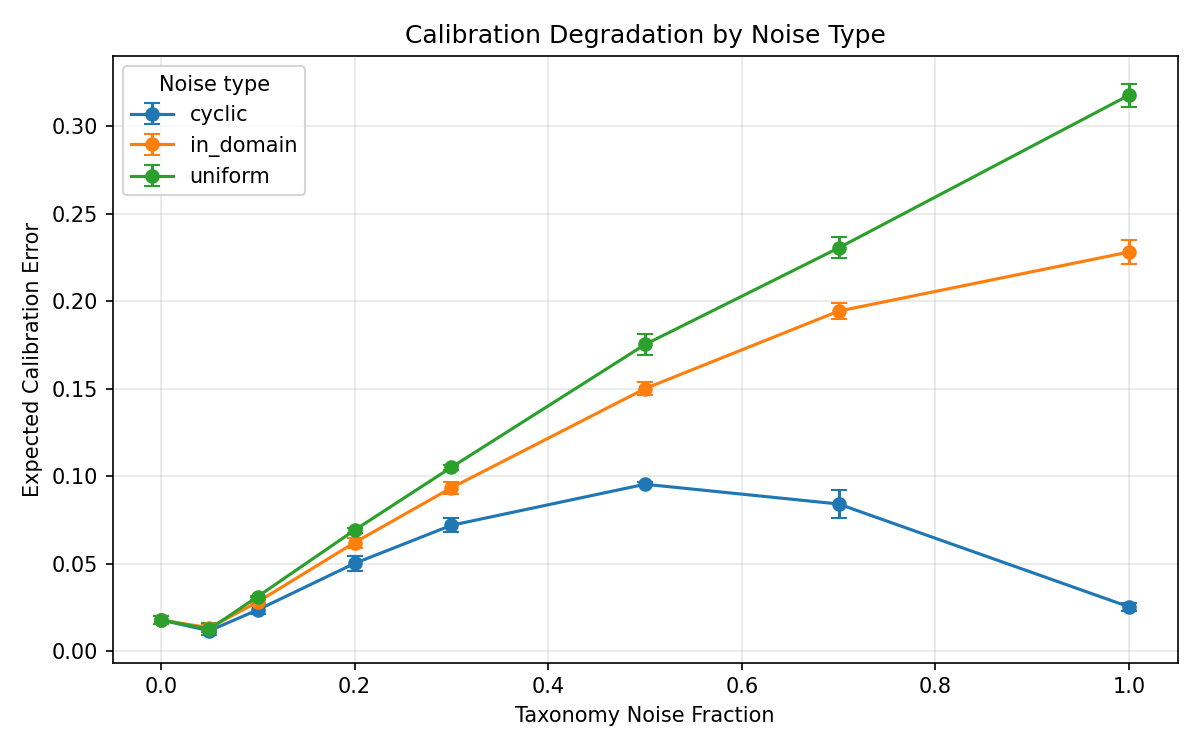
\includegraphics[width=0.88\textwidth]{ece_by_noise_type.png}
\caption{Expected calibration error as parent-label corruption increases.}
\label{fig:ece}
\end{figure}

Second, structured noise changes the semantic severity of errors. Figure
\ref{fig:hierdist} plots hierarchical distance against noise fraction. Cyclic
noise causes the mean distance to grow sharply, indicating that errors move
from near misses within related parents toward more severe cross-parent or
cross-domain confusions. Uniform noise leaves hierarchical distance relatively
stable, which is consistent with its smaller effect on leaf accuracy.

\begin{figure}
\centering
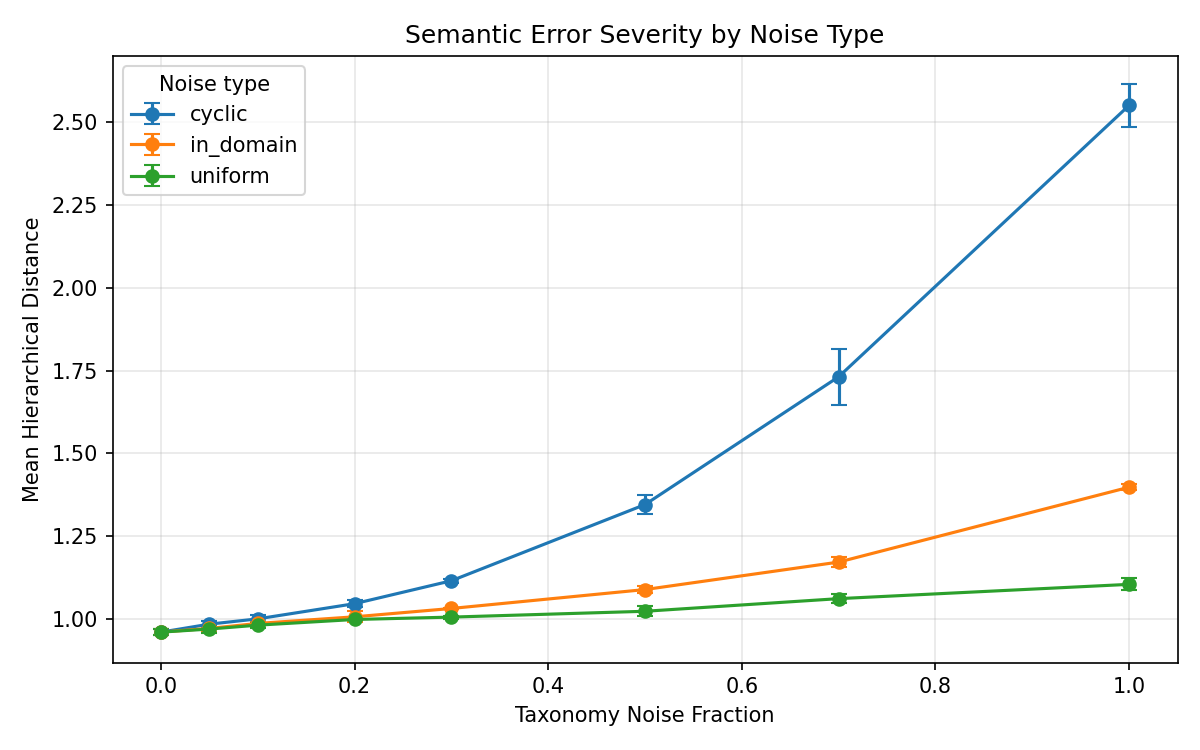
\includegraphics[width=0.88\textwidth]{hier_distance_by_noise_type.png}
\caption{Mean hierarchical distance, where larger values indicate semantically more severe errors.}
\label{fig:hierdist}
\end{figure}

\subsection{Parent Collapse Versus Leaf Robustness}
Figure~\ref{fig:leafparent} compares parent accuracy and leaf accuracy across
all noisy hierarchy-aware runs. The scatter shows that parent accuracy can
collapse before leaf accuracy fully collapses. Uniform full corruption yields
near-zero parent accuracy while leaf accuracy remains near 71\%. In contrast,
cyclic corruption produces both low parent accuracy and a major leaf-accuracy
drop. This supports the interpretation that parent-head failure is not by
itself sufficient to destroy the leaf task; the damage is largest when the
wrong parent signal is coherent enough to reshape the leaf boundary.

\begin{figure}
\centering
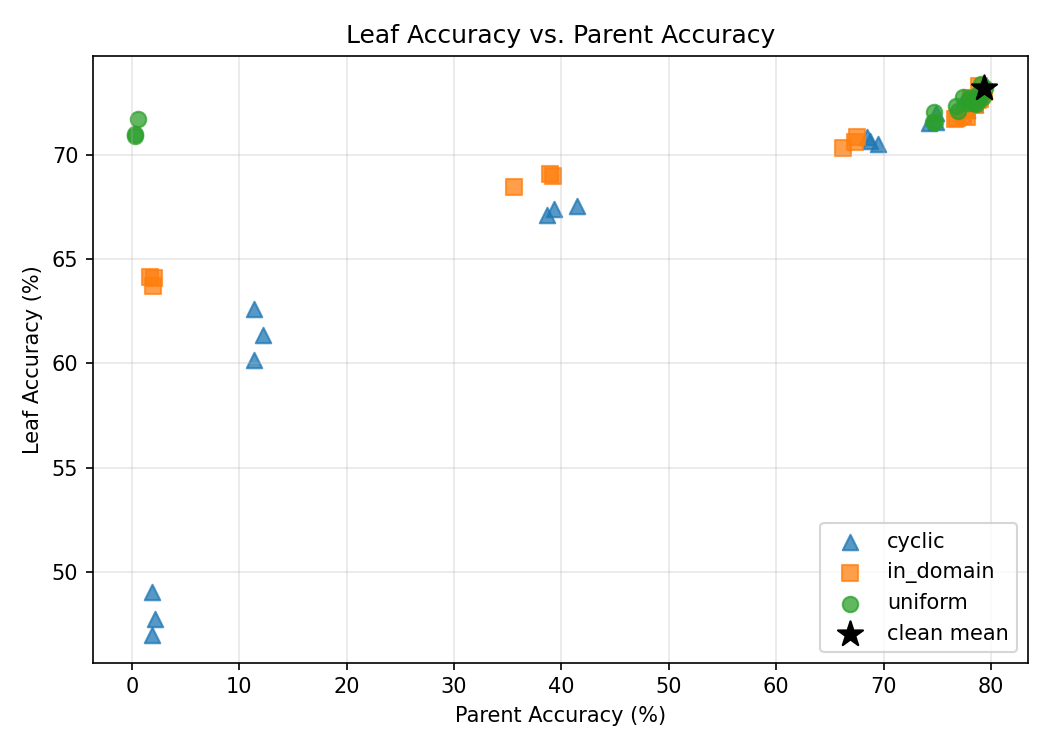
\includegraphics[width=0.82\textwidth]{leaf_vs_parent_accuracy.png}
\caption{Relationship between parent accuracy and leaf accuracy across noisy hierarchy-aware runs.}
\label{fig:leafparent}
\end{figure}

\subsection{Per-Parent Sensitivity}
Aggregate degradation curves do not show which parts of the taxonomy are most
fragile. Figure~\ref{fig:heatmap} presents per-parent leaf accuracy under
cyclic noise, the most damaging corruption type. The heatmap shows that
accuracy degradation is not uniform. Parent groups such as aquatic mammals and
small mammals become much darker at high corruption, while large man-made
outdoor things and vehicles remain comparatively strong. This suggests that
taxonomy noise interacts with visual separability: visually distinctive parent
groups can retain useful leaf boundaries even when parent supervision is
incorrect, whereas visually confusable animal groups are more vulnerable.

\begin{figure}
\centering
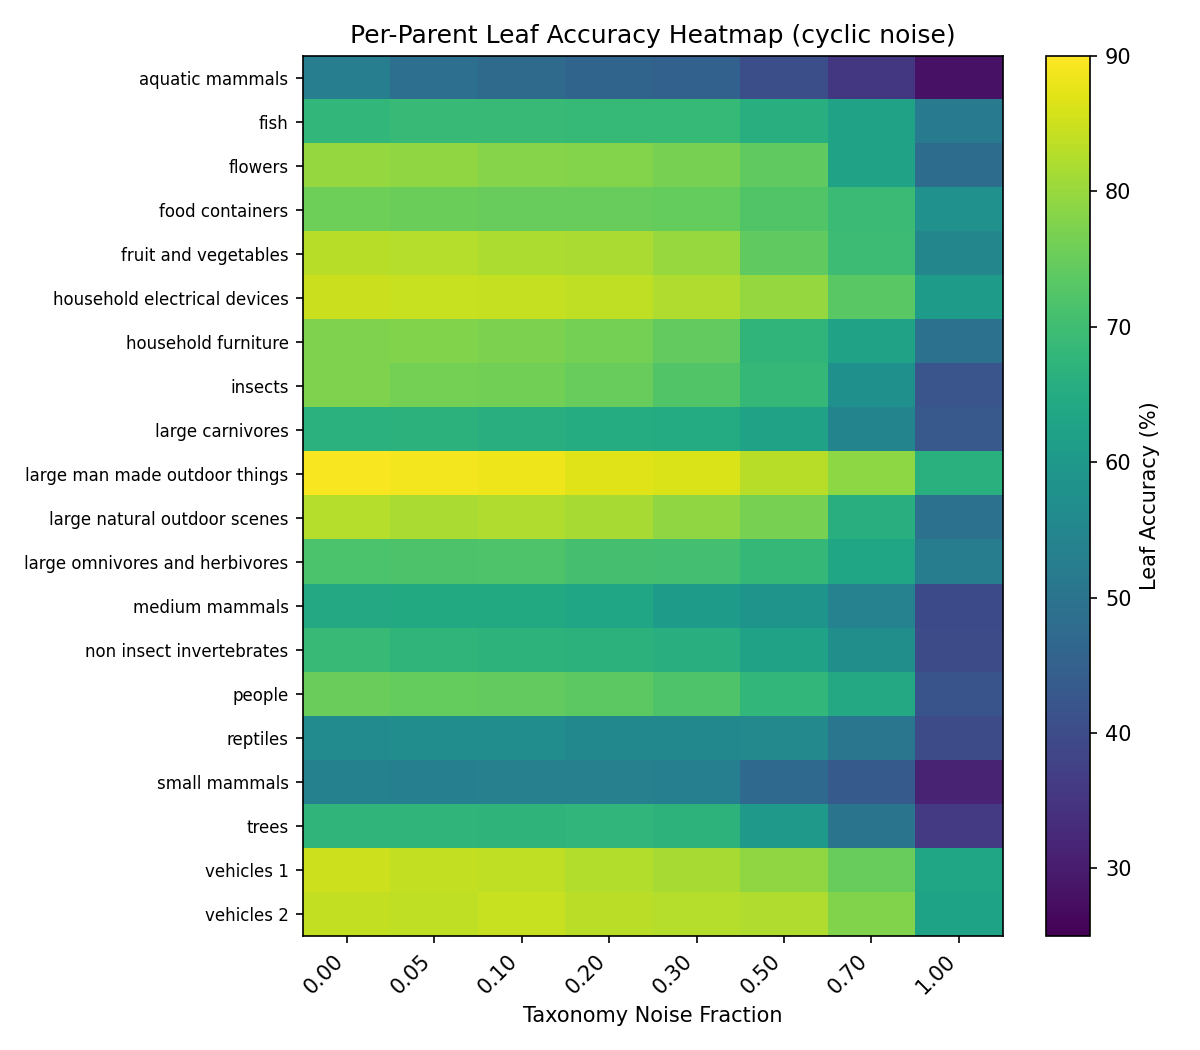
\includegraphics[width=0.86\textwidth]{per_parent_heatmap_cyclic.png}
\caption{Per-parent leaf accuracy under cyclic taxonomy noise. Each cell averages over three seeds.}
\label{fig:heatmap}
\end{figure}

\subsection{Interpretation}
The results support two main interpretations. First, hierarchy-aware adaptation
is not automatically superior to flat adaptation when leaf labels are abundant.
On CIFAR-100, clean hierarchy supervision mainly improves secondary metrics
such as hierarchical distance and calibration. Second, taxonomy-noise
robustness depends heavily on whether errors are independent or structured.
Uniform corruption distributes wrong parent labels across the taxonomy, so the
auxiliary signal is noisy but not consistently misleading in one direction.
In-domain corruption is semantically plausible and therefore more likely to
interfere with boundaries among related visual groups. Cyclic corruption is
coherent and systematic; the model receives a stable but wrong mapping between
leaves and parents, which strongly damages the coupled leaf-to-parent
consistency objective.

\section{Reproducibility}
The full source code, experiment scripts, generated results, figures, and
Springer-format report are maintained in the GitHub repository:
\begin{center}
\url{https://github.com/manuvikash/VLM-finetune}
\end{center}
The committed experiment artifacts include the aggregate result JSON, the
per-parent metric CSV, the noise-type summary CSV, and all figures used in this
paper.
The generated JPEG image directory is intentionally ignored by git because it
contains 60,000 reproducible CIFAR-derived files. It can be regenerated from
the committed manifests and builder script.

The main commands are:
\begin{verbatim}
python build_dataset.py
  --num-coarse 20 --per-class 0
  --use-test-split

python feature_sweep.py
  --epochs 30 --seeds 42 123 456
  --noise-fractions 0.0 0.05 0.1 0.2
  0.3 0.5 0.7 1.0
  --noise-types uniform in_domain cyclic
  --lambda-parent 1.0
  --consistency-weight 0.8 --lr 0.001

python analysis.py
  --export-csv results
  --plot --plot-dir figures
  --per-parent-csv runs/per_parent_metrics.csv
\end{verbatim}

\section{Conclusion}
This paper evaluated hierarchy-aware CLIP adaptation under controlled taxonomy
noise. On the full CIFAR-100 hierarchy, clean hierarchy-aware adaptation
matches flat adaptation in leaf accuracy and modestly improves hierarchical
distance and calibration. The main finding is that robustness depends strongly
on the type of taxonomy error. Uniform parent-label noise is largely tolerated,
but structured noise can severely harm fine-grained recognition. At full
corruption, uniform noise retains 71.19\% leaf accuracy, in-domain noise drops
to 63.97\%, and cyclic systematic noise drops to 47.93\%. Additional
visualizations show that calibration can degrade even when accuracy is stable,
hierarchical distance exposes semantically worse mistakes under systematic
noise, parent accuracy can collapse before leaf accuracy does, and different
parent groups have different sensitivity to taxonomy corruption.

For practical VLM fine-tuning, the most important question is therefore not
only how many parent labels are noisy, but whether the errors encode a coherent
wrong taxonomy. Future work should repeat the study with full end-to-end
backbone fine-tuning, larger VLMs, deeper real-world taxonomies, and asymmetric
noise processes based on observed annotation errors. Another useful direction
is to design hierarchy-aware losses that can detect and down-weight suspicious
parent targets while preserving the benefits of clean hierarchical supervision.

\begin{thebibliography}{7}

\bibitem{radford2021clip}
A. Radford et al., ``Learning transferable visual models from natural language
supervision,'' in \emph{Proc. ICML}, 2021.

\bibitem{ilharco2021openclip}
G. Ilharco et al., ``OpenCLIP,'' 2021. [Online]. Available:
\url{https://github.com/mlfoundations/open_clip}

\bibitem{krizhevsky2009learning}
A. Krizhevsky, ``Learning multiple layers of features from tiny images,''
University of Toronto, Tech. Rep., 2009.

\bibitem{guo2017calibration}
C. Guo, G. Pleiss, Y. Sun, and K. Q. Weinberger, ``On calibration of modern
neural networks,'' in \emph{Proc. ICML}, 2017.

\bibitem{silla2011survey}
C. N. Silla Jr. and A. A. Freitas, ``A survey of hierarchical classification
across different application domains,'' \emph{Data Mining and Knowledge
Discovery}, vol. 22, no. 1--2, pp. 31--72, 2011.

\bibitem{patrini2017noise}
G. Patrini, A. Rozza, A. K. Menon, R. Nock, and L. Qu, ``Making deep neural
networks robust to label noise: A loss correction approach,'' in
\emph{Proc. CVPR}, 2017, pp. 1944--1952.

\bibitem{geirhos2020shortcut}
R. Geirhos, J.-H. Jacobsen, C. Michaelis, R. Zemel, W. Brendel, M. Bethge,
and F. A. Wichmann, ``Shortcut learning in deep neural networks,''
\emph{Nature Machine Intelligence}, vol. 2, pp. 665--673, 2020.

\end{thebibliography}

\end{document}
